\documentclass[a4paper,12pt]{article}
\usepackage[a4paper,top=1.3cm,bottom=2cm,left=1.5cm,right=1.5cm,marginparwidth=0.75cm]{geometry}
\usepackage{cmap}
\usepackage{mathtext}
\usepackage[T2A]{fontenc}
\usepackage[utf8]{inputenc}
\usepackage[english,russian]{babel}
\usepackage{siunitx}
\usepackage{enumitem}
\usepackage{placeins}

\usepackage{graphicx}
\usepackage{amsmath}

\usepackage{wrapfig}
\usepackage{tabularx}
\usepackage{multirow}

\usepackage{hyperref}
\usepackage[rgb]{xcolor}
\hypersetup{colorlinks=true,urlcolor=blue}
\usepackage{siunitx}
\usepackage{amsmath,amsfonts,amssymb,amsthm,mathtools}
\usepackage{mathtools}
\usepackage{icomma}
\mathtoolsset{showonlyrefs=false}
\usepackage{euscript}
\usepackage{mathrsfs}
\DeclareMathOperator{\sgn}{\mathop{sgn}}
\newcommand*{\hm}[1]{#1\nobreak\discretionary{}
{\hbox{$\mathsurround=0pt #1$}}{}}

%%% Заголовок
\newcommand\labname{Изучение спектров атомов водорода и дейтерия}
\newcommand\labnumber{2.2}


\author{Макаров Лев Евгеньевич}
\title{Лабораторная работа №\labnumber

\labname
}

\date{\today}

\makeatletter
\AddEnumerateCounter{\asbuk}{\russian@asbuk@alph}{щ} % section 8.1
\makeatother


\begin{document}


\begin{titlepage}
	\begin{center}
		{\large МОСКОВСКИЙ ФИЗИКО-ТЕХНИЧЕСКИЙ ИНСТИТУТ (НАЦИОНАЛЬНЫЙ ИССЛЕДОВАТЕЛЬСКИЙ УНИВЕРСИТЕТ)}
	\end{center}
	\begin{center}
		{\large Физтех-школа фотоники, электроники и молекулярной физики}
	\end{center}
	
	
	\vspace{4.5cm}
	{\huge
		\begin{center}
			{\bf Отчёт о выполнении лабораторной работы \labnumber}\\
			\labname
		\end{center}
	}
	\vspace{2cm}
	\begin{flushright}
		{\LARGE Автор:\\ Макаров Лев Евгеньевич \\
			\vspace{0.2cm}
			Б04-306}
	\end{flushright}
	\vspace{8cm}
	\begin{center}
		Долгопрудный 2025
	\end{center}
\end{titlepage}

\section{Введение}

\textbf{Цель работы:} 
\begin{enumerate}
	\item Исследовать спектральные закономерности в оптических спектрах водорода и дейтерия
    \item По результатам измерений вычисляются постоянные Ридберга для этих двух изотопов водорода, их потенциалы ионизации, изотопические сдвиги линий
\end{enumerate}


\section{Теоретические сведения}

Атом водорода является простейшей атомной системой; для него уравнение Шредингера может быть решено точно. Поэтому спектр атома водорода является предметом тщательного экспериментального и теоретического исследования.

Объяснение структуры спектра излучения атомов требует знания схемы атомных энергетических уровней. Для атома водорода и водородоподобных (одноэлектронных) атомов определение энергетических уровней значительно упрощается, так как квантово-механическая задача об относительном движении электрона (заряд \(-e\), масса \(m_e\)) и ядра (заряд \(Ze\), масса \(M\)) сводится к задаче о движении частицы с эффективной массой \(\mu = m_e M / (m_e + M)\) в кулоновском поле \(-Ze^2 / r\).

Длины волн спектральных линий водородоподобного атома описываются \textbf{обобщенной формулой Бальмера}:

\begin{equation}\label{eq:balmer}
    \frac{1}{\lambda_{mn}} = R Z^2 \left( \frac{1}{n^2} - \frac{1}{m^2} \right),
\end{equation}

где \(R\) — постоянная Ридберга, \(Z\) — зарядовое число ядра, а \(m\) и \(n\) — целые числа (\(m > n\)).

Для объяснения спектра атома водорода Нильс Бор в 1913 г. предложил теорию атома, основанную на трех постулатах:
\begin{enumerate}
    \item Существуют только некоторые стационарные орбиты, при движении по которым электрон не излучает энергии.
    \item Момент количества движения электрона на стационарной орбите квантуется: \(L = n\hbar\), где \(n=1,2,3\ldots\)
    \item Излучение или поглощение энергии происходит при переходе атома между стационарными состояниями, причем частота излучения определяется разностью энергий: \(h\nu = E_m - E_n\).
\end{enumerate}

Использование этих постулатов позволяет определить возможные энергетические состояния водородоподобного атома:

\begin{equation}\label{eq:energy_levels}
    E_n = -\frac{2\pi^2 \mu e^4 Z^2}{h^2} \cdot \frac{1}{n^2} = -R \frac{Z^2}{n^2},
\end{equation}

где \(\mu\) — приведенная масса системы электрон-ядро.

В данной работе изучается \textbf{серия Бальмера}, линии которой лежат в видимой области спектра и соответствуют переходам на уровень с \(n=2\). Первые четыре линии этой серии (\(m = 3, 4, 5, 6\)) обозначаются символами \(H_\alpha\) (красная), \(H_\beta\) (зелено-голубая), \(H_\gamma\) (фиолетово-синяя), \(H_\delta\) (фиолетовая).

Постоянная Ридберга \(R\) в формуле (\ref{eq:balmer}) зависит от приведенной массы \(\mu\):

\begin{equation}\label{eq:rydberg_mass}
    R = \frac{2\pi^2 \mu e^4}{c h^3}.
\end{equation}

Поскольку приведенная масса для разных изотопов водорода (протия \(^1H\) и дейтерия \(^2H\)) различна, различаются и их постоянные Ридберга (\(R_H\) и \(R_D\)), а следовательно, и длины волн соответствующих спектральных линий. Это явление называется \textbf{изотопическим сдвигом}. Величина относительного сдвига между линиями водорода и дейтерия определяется выражением:

\begin{equation}\label{eq:isotope_shift}
    \frac{\Delta \lambda}{\lambda} \approx \frac{m_e}{2 M_p},
\end{equation}

где \(M_p\) — масса протона.

\section{Экспериментальная установка}

Экспериментальная установка состоит из двух основных частей.

\subsection{Часть I. Измерение длин волн серии Бальмера}

Для измерения длин волн спектральных линий в работе используется стеклянно-призменный монохроматор-спектрометр УМ-2, предназначенный для спектральных исследований в диапазоне от 0,38 до 1,00 мкм.

\FloatBarrier
\begin{figure}[h]
    \begin{center}
        
\includegraphics[width = 0.45\textwidth]{pics/ustan_1.png}
        \caption{Устройство монохроматора УМ-2}
    \label{pic:ustan_1}
    \end{center}
\end{figure}
\FloatBarrier

Основные элементы монохроматора УМ-2 (рис. \ref{pic:ustan_1}):
\begin{enumerate}
    \item \textbf{Входная щель}, снабженная микрометрическим винтом для регулировки ширины (0,01–0,03 мм).
    \item \textbf{Коллиматорный объектив}, фокусирующий свет на призму.
    \item \textbf{Сложная спектральная призма}, состоящая из трех склеенных призм (П1, П2, П3). Призмы П1 и П2 изготовлены из тяжелого флинта (большая дисперсия), призма П3 — из крона. Лучи отражаются от её гипотенузной грани и поворачиваются на \(90^\circ\), что позволяет складывать дисперсии призм П1 и П2.
    \item \textbf{Поворотный столик} с призмой, вращающийся вокруг вертикальной оси при помощи микрометрического винта с отсчетным барабаном.
    \item \textbf{Зрительная труба}, состоящая из объектива и окуляра. В фокальной плоскости объектива расположено острие указателя, совмещаемое с центром спектральной линии для отсчета её положения по барабану.
    \item \textbf{Оптическая скамья} с рейтерами для источника света и конденсора, служащего для концентрации света на входной щели.
    \item \textbf{Пульт управления} для питания источников света и осветительной системы.
\end{enumerate}




В качестве источника света используется \textbf{водородная лампа} Н-образной формы, питаемая от источника высокого напряжения. Наибольшая яркость спектра достигается при освещении от торца горизонтальной части трубки (капилляра). Для увеличения яркости атомарных линий в газ добавляют пары воды, которые разлагаются в разряде.

Перед измерениями спектрометр необходимо \textbf{проградуировать}. Для этого используются эталонные источники света:
\begin{itemize}
    \item \textbf{Ртутная лампа ПРК-4} — для коротковолновой части спектра.
    \item \textbf{Неоновая лампа} — для длинноволновой и средней части спектра.
\end{itemize}

Строится градуировочный график \(\lambda = f(N)\), где \(N\) — отсчет по барабану.

\subsection{Часть II. Измерение изотопического сдвига}

Для обнаружения и измерения малого изотопического сдвига между линиями водорода и дейтерия используется спектральный прибор с более высокой разрешающей способностью — \textbf{отражательная дифракционная решетка}, установленная на гониометре Г-1,5.

Основные элементы установки (рис. \ref{pic:ustan_2}):
\begin{enumerate}
    \item \textbf{Источник света}: водородно-дейтериевая лампа ДВС-25.
    \item \textbf{Гониометр Г-1,5}, включающий:
    \begin{itemize}
        \item Зрительную трубу.
        \item Коллиматор со щелью.
        \item Столик с установленной дифракционной решеткой.
        \item Микроскоп для отсчета углов.
    \end{itemize}
    \item \textbf{Отражательная дифракционная решетка}.
\end{enumerate}

\FloatBarrier
\begin{figure}[h]
    \begin{center}
        
\includegraphics[width = 0.45\textwidth]{pics/ustan_2.png}
        \caption{Схема экспериментальной установки}
    \label{pic:ustan_2}
    \end{center}
\end{figure}
\FloatBarrier

Градуировка производится по спектру неоновой лампы. Измеряются углы отклонения для линий водорода (\(H_\alpha\)) и дейтерия (\(D_\alpha\)) в первом порядке дифракции. По разнице их положений определяется изотопический сдвиг \(\Delta \lambda\), который сравнивается с расчетным значением по формуле (\ref{eq:isotope_shift}).


\section{Результаты измерений и обработка данных}

\subsection*{I. Подготовка приборов к работе}

\begin{enumerate}
    \item Ознакомимся с устройством и принципом работы спектрометра.
    \item Отцентрируем систему.
    \item Перемещая источник вдоль оптической оси, получим резкое изображение источника в центре колпачка. Закрепим рейтеры.
    \item Включим подсветку окуляра. Вращая глазную линзу окуляра, настроимся на резкое изображение спектра. Реостатом отрегулируем яркость указателя.
    \item Подведем к указателю одну из ярких линий неона. Вращая коллиматор сделаем ее четкой.
    \item Подберем ширину щели: начнем открывать и после момента открытия повернем винт еще на 0.07 мм.
    \item Убедимся, что барабана хватает для измерения всех линий.
    \item Подберем положение коллиматора так, чтобы отсутствовал параллакс при смещении глаза влево-вправо.
\end{enumerate}


\subsection*{II. Градуировка спектрометра}

\begin{enumerate}
    \item Проградуируем спектрометр по спектру неона. Погрешность измерений на барабане считаем $\sigma_\varphi = 1$ град. Точность с которой известна длина волны линий: $\sigma_\lambda = 0.5$ \AA.
\end{enumerate}

Замерим положение линий неона и запишем в таблицу \ref{table:grad}.

\begin{enumerate}[resume]
    \item Аналогично сделаем для линий ртути.
\end{enumerate}



\begin{table}[!h]
    \centering
    \begin{minipage}{0.48\textwidth}
        \centering
        \begin{tabular}{l|l|l}
            \hline
            $\lambda$, \AA & $\varphi$, град & лампа \\ \hline
            5331 & 1834 & Ne \\
            5341 & 1842 & Ne \\
            5401 & 1884 & Ne \\
            5852 & 2145 & Ne \\
            5882 & 2158 & Ne \\
            5945 & 2189 & Ne \\
            5976 & 2203 & Ne \\
            6030 & 2229 & Ne \\
            6074 & 2249 & Ne \\
            6096 & 2258 & Ne \\
            6143 & 2278 & Ne \\
            6164 & 2288 & Ne \\
            6217 & 2308 & Ne \\
            6267 & 2328 & Ne \\ \hline
        \end{tabular}
    \end{minipage}%
    \hfill
    \begin{minipage}{0.48\textwidth}
        \centering
        \begin{tabular}{l|l|l}
            \hline
            $\lambda$, \AA & $\varphi$, град & лампа \\ \hline
            6305 & 2343 & Ne \\
            6334 & 2356 & Ne \\
            6383 & 2374 & Ne \\
            6402 & 2381 & Ne \\
            6507 & 2418 & Ne \\
            6533 & 2426 & Ne \\
            6599 & 2450 & Ne \\
            6678 & 2478 & Ne \\
            6717 & 2489 & Ne \\
            6929 & 2554 & Ne \\
            7032 & 2585 & Ne \\
            5791 & 2112 & Hg \\
            5770 & 2100 & Hg \\
            5461 & 1921 & Hg \\
            4916 & 1504 & Hg \\ \hline
        \end{tabular}
    \end{minipage}
    \caption{Градуировочные значения для спектрометра}
    \label{table:grad}
\end{table}


\FloatBarrier
\clearpage

\subsection*{III. Спектр водорода}

\begin{enumerate}
    \item Установим на скамью водородную лампу и включим ее в сеть.
    \item Замерим положение линий $H_\alpha$, $H_\beta$, $H_\gamma$ и $H_\delta$. Запишем результаты в таблицу \ref{table:H_measurements}. Линию $H_\delta$ измерить не получилось.
\end{enumerate}


\subsection*{IV. Спектр йода}

\begin{enumerate}
    \item Ознакомимся с принципом измерения спектра йода.
    \item Установим на скамью кювету с йодом и лампу накаливания. Включим лампу и отценрируем установку.
    \item Убедимся, что спектр поглощения хорошо виден. Уменьшим ширину щели так, чтобы было лучше видно.
    \item Измерим положения: самой длинноволновой линии поглощения ($h \nu_{1,0}$), шестой по счету от предыдущей ($h \nu_{1,5}$) и границы, где начинается сплошной спектр ($h \nu_\text{гр}$). Измерения запишем в таблицу \ref{table:I_measurements}
\end{enumerate}

\subsection*{V. Обработка результатов}

\begin{enumerate}
    \item Построим градуировочную кривую. Изображена на рис. \ref{pic:grad_graph}.
\end{enumerate}

Аппроксимируем градуировочную кривую формулой:

\begin{equation*}
    \lambda (\varphi) = \lambda_0 + \cfrac{C}{\varphi - \varphi_0}
\end{equation*}

Погрешность при таком вычислении:

\begin{multline*}
    \sigma_\lambda = \sqrt{\left( \cfrac{\partial \lambda}{\partial \lambda_0}\right)^2 \sigma_{\lambda_0}^2 + \left(\cfrac{\partial \lambda}{\partial C}\right)^2 \sigma_{C}^2 + \left( \cfrac{\partial \lambda}{\partial \varphi_0}\right)^2\sigma_{\varphi_0}^2 + \left( \cfrac{\partial \lambda}{\partial \varphi}\right)^2 \sigma_{\varphi}^2} = \\ = \sqrt{\sigma_{\lambda_0}^2 + \left(\cfrac{\lambda - \lambda_0}{C}\right)^2 \sigma_{C}^2 + \left( \cfrac{\lambda - \lambda_0}{\varphi - \varphi_0}\right)^2 (\sigma_{\varphi_0}^2 + \sigma_{\varphi}^2) }
\end{multline*}

\clearpage

\FloatBarrier
\begin{figure}[!ht]
	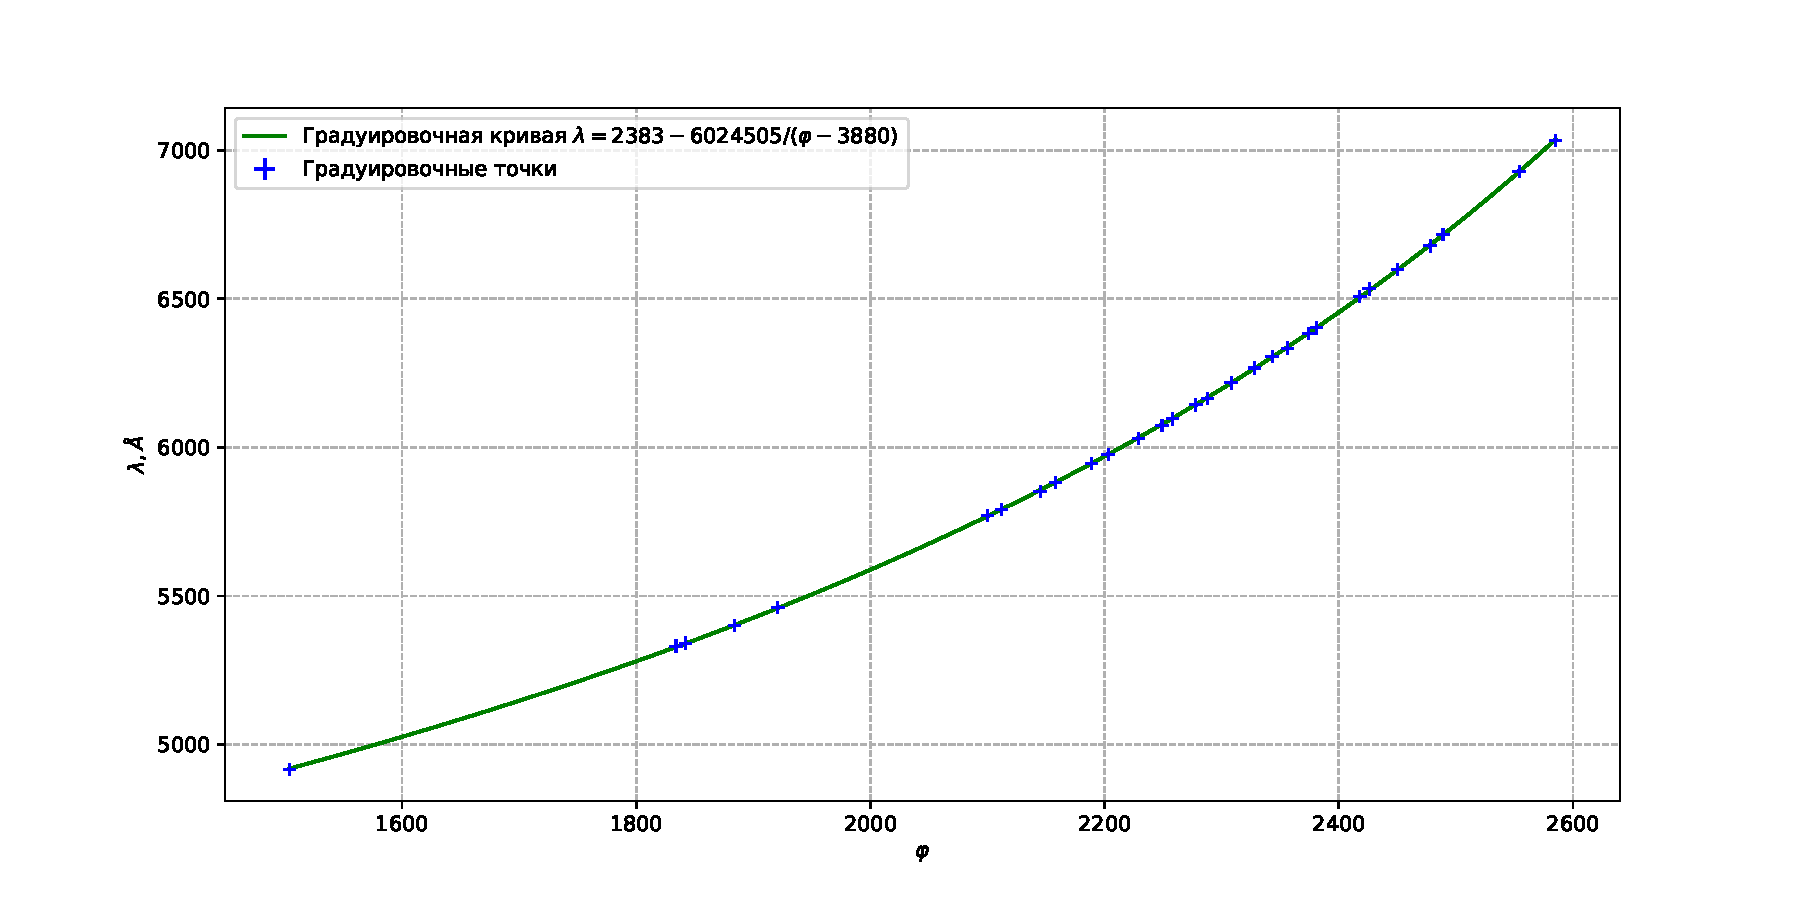
\includegraphics[width=1.1\textwidth]{pics/grad_graph.pdf}
	\caption{\textit{Градуировочная кривая спектрометра}}
	\label{pic:grad_graph}
\end{figure}
\FloatBarrier

Параметры функции аппроксимации:

\begin{equation*}
    \lambda_0 = (23826 \pm 2) \cdot 10 \ \text{\AA}
\end{equation*}
\begin{equation*}
    \varphi_0 = (3880 \pm 9) \ \text{град}
\end{equation*}
\begin{equation*}
    c = -(60245052380 \pm 7) \cdot 10^4 \ \text{\AA}
\end{equation*}

\begin{enumerate}[resume]
    \item Определим длины волн линий водорода (и их погрешность) и запишем в таблицу \ref{table:H_measurements}.
\end{enumerate}


\begin{table}[h]
    \centering
    \begin{tabular}{l|l|l|l|l|l}
        \hline
        линия      & цвет            & $\varphi$, град & n & $\lambda$, \AA & $\sigma_\lambda$, \AA \\ \hline
        $H_\alpha$ & Красный         & 2440            & 3 & 6570           & 20 \\
        $H_\beta$  & Зелено-голубой  & 1450            & 4 & 4860           & 23 \\
        $H_\gamma$ & Фиолетово-синий & 820             & 5 & 4350           & 27 \\
        $H_\delta$ & Фиолетовый      & -               & 6 & -              & -  \\ \hline
    \end{tabular}
    \caption{Измерение линий водорода}
    \label{table:H_measurements}
\end{table}

\begin{enumerate}[resume]
    \item Убедимся в том, что отношение длин волн водородных линий соответствует формуле сериальной закономерности:
\end{enumerate}

\begin{equation*}
    \cfrac{1}{\lambda_{mn}} = R Z^2 \left( \cfrac{1}{n^2} - \cfrac{1}{m^2} \right) \implies \cfrac{\lambda_{m_1 n}}{\lambda_{m_2 n}} = \cfrac{1 - \cfrac{n^2}{m_1^2}}{1 - \cfrac{n^2}{m_2^2}}
\end{equation*}

Посчитаем теоретические и экспериментальные значения и запишем в таблицу \ref{table:serial_formula_check_2}.


\FloatBarrier
\begin{table}[!h]
    \centering
    \begin{minipage}{0.48\textwidth}
        \centering
        \begin{tabular}{|l|lll|}
            \hline
            ~ & 3      & 4      & 5      \\ \hline
            3 & 1.0000 & 0.7407 & 0.6613 \\ 
            4 & 1.3500 & 1.0000 & 0.8928 \\
            5 & 1.5120 & 1.1200 & 1.0000 \\ \hline
        \end{tabular}
        \caption{Теоретические значения}
        \label{table:serial_formula_check_1}
    \end{minipage}%
    \hfill
    \begin{minipage}{0.48\textwidth}
        \centering
        \begin{tabular}{|l|lll|}
            \hline
            ~ & 3     & 4     & 5     \\ \hline
            3 & 1.000 & 0.740 & 0.663 \\ 
            4 & 1.351 & 1.000 & 0.895 \\
            5 & 1.51  & 1.117 & 1.000 \\ \hline
        \end{tabular}
        \caption{Экспериментальные значения}
        \label{table:serial_formula_check_2}
    \end{minipage}%
    \begin{minipage}{0.48\textwidth}
        \centering
        \begin{tabular}{|l|lll|}
            \hline
            ~ & 3     & 4     & 5     \\ \hline
            3 & 0.004 & 0.004 & 0.005 \\ 
            4 & 0.008 & 0.007 & 0.007 \\
            5 & 0.01  & 0.008 & 0.009 \\ \hline
        \end{tabular}
        \caption{Погрешности экспериментальных значений}
        \label{table:serial_formula_check_3}
    \end{minipage}
\end{table}
\FloatBarrier


Как видно соотношения выполняются.

\begin{enumerate}[resume]
    \item Для измеренных линий водорода посчитаем постоянную Ридберга и ее погрешность. Запишем результаты вычислений в таблицу \ref{table:H_Ridberg}
\end{enumerate}


\begin{table}[h]
    \centering
    \begin{tabular}{l|l|l|l|l}
        \hline
        линия      & $R_H$, $\text{см}^{-1}$ & $\sigma_{R_H}$, $\text{см}^{-1}$ & $R_H$, эВ & $\sigma_{R_H}$, эВ \\ \hline
        $H_\alpha$ & $1.096 \cdot 10^7$ & $3 \cdot 10^4$ & 13.57 & 0.04 \\
        $H_\beta$  & $1.096 \cdot 10^7$ & $5 \cdot 10^4$ & 13.57 & 0.06 \\
        $H_\gamma$ & $1.094 \cdot 10^7$ & $7 \cdot 10^4$ & 13.54 & 0.08 \\ \hline
    \end{tabular}
    \caption{Подсчет постоянной Ридберга для измеренных линий водорода}
    \label{table:H_Ridberg}
\end{table}

Тогда значение постоянной возьмем как среднее: $R_H^\text{эксп} = \langle R_H \rangle = 13.56$ эВ.

Случайная погрешность измерения: $\sigma_{R_H}^\text{случ} = \sqrt{\frac{1}{N(N - 1)} \sum \left(R_H - \overline{R_H}\right)^2} = 0.01$ эВ

Тогда экспериментальное значение (с учетом погрешности измерения):

\begin{equation*}
    R_H^\text{эксп} = (13.56 \pm 0.08) \ \text{эВ} \ \ \ \ \ R_H^\text{теор} = 13.6 \ \text{эВ}
\end{equation*}

Как видно экспериментальное значение совпадает с теоретическим в пределах погрешности.

\begin{enumerate}[resume]
    \item Посчитаем по градуировочной кривой длины волн для линий йода и соотвествующую им энергию $h \nu$. Запишем результаты измерений в таблицу \ref{table:I_measurements}.
\end{enumerate}

\begin{table}[h]
    \centering
    \begin{tabular}{l|l|l|l|l|l}
        \hline
        линия             & $\varphi$, град & $\lambda$, \AA & $\sigma_\lambda$, \AA & $h\nu$, эВ & $\sigma_{h\nu}$, эВ \\ \hline
        $h \nu_{1,0}$     & 2235 & 6050 & 20 & 2.051 & 0.007 \\
        $h \nu_{1,5}$     & 2128 & 5820 & 21 & 2.130 & 0.008 \\
        $h \nu_\text{гр}$ & 2262 & 6110 & 20 & 2.031 & 0.007 \\ \hline
    \end{tabular}
    \caption{Измерение спектра йода и подсчет длин волн}
    \label{table:I_measurements}
\end{table}

\begin{enumerate}[resume]
    \item Вычислим энергию колебательного кванта возбужденного состояния молекулы йода.
\end{enumerate}

\begin{equation*}
    h \nu_2 = \frac{h \nu_{1,5} - h \nu_{1,0}}{5} = (0.016 \pm 0.002) \ \text{эВ}
\end{equation*}

\clearpage
\begin{enumerate}[resume]
    \item Используя известные значения для энергии колебательного кванта основного состояния $h \nu_1 = 0.027$ эВ и энергии возбуждения атома $E_A = 0.94$ эВ (Погрешность считаем как половину последнего известного разряда), посчитаем
    \begin{enumerate}[label=\asbuk*.]
        \item Энергию электронного перехода:
    \end{enumerate}
    
\begin{equation*}
    h \nu_{\text{эл}} = h \nu_{1,0} - \cfrac{1}{2}h \nu_2 + \cfrac{3}{2} h \nu_1
\end{equation*}

Погрешность $\sigma_{h \nu_{\text{эл}}} = \sqrt{ \sigma_{h \nu_{1,0}}^2 + \cfrac{1}{4} \sigma_{h \nu_2}^2 + \cfrac{9}{4} \sigma_{h \nu_1}^2 }$

\begin{equation*}
    h \nu_{\text{эл}} = (2.08 \pm 0.01) \ \text{эВ}
\end{equation*}

    \begin{enumerate}[label=\asbuk*.,resume]
        \item Энергию диссоциации молекулы в основном состоянии:
    \end{enumerate}

\begin{equation*}
    D_1 = h \nu_\text{гр} - E_A
\end{equation*}

Погрешность: $\sigma_{D_1} = \sqrt{\sigma_{h \nu_\text{гр}}^2 + \sigma_{E_A}^2}$

\begin{equation*}
    D_1 = (1.09 \pm 0.01) \ \text{эВ}
\end{equation*}


    \begin{enumerate}[label=\asbuk*.,resume]
        \item Энергию диссоциации молекулы в возбужденном состоянии:
    \end{enumerate}

\begin{equation*}
    D_2 = h \nu_\text{гр} - h \nu_\text{эл}
\end{equation*}

Погрешность: $\sigma_{D_2} = \sqrt{\sigma_{h \nu_\text{гр}}^2 + \sigma_{h \nu_\text{эл}}^2}$

\begin{equation*}
    D_2 = -(0.05 \pm 0.01) \ \text{эВ}
\end{equation*}

\end{enumerate}


\section{Выводы}

\begin{enumerate}
    \item Была получена градуировочная кривая и исследованы спектры водорода и йода.
    \item Была посчитана постоянная Ридберга для водорода и потенциалы ионизации для йода. 

    Которые не совпали с табличными данными. Скорее всего из-за неправильного измерения $h \nu_{\text{гр}}$, ведь четкой границы не видно в глазок.
\end{enumerate}


\end{document}
